\begin{anexosenv}

\partanexos

\chapter{Telas da Aplicação}
\label{chap:telas}

\begin{figure}[H]
    \centering
    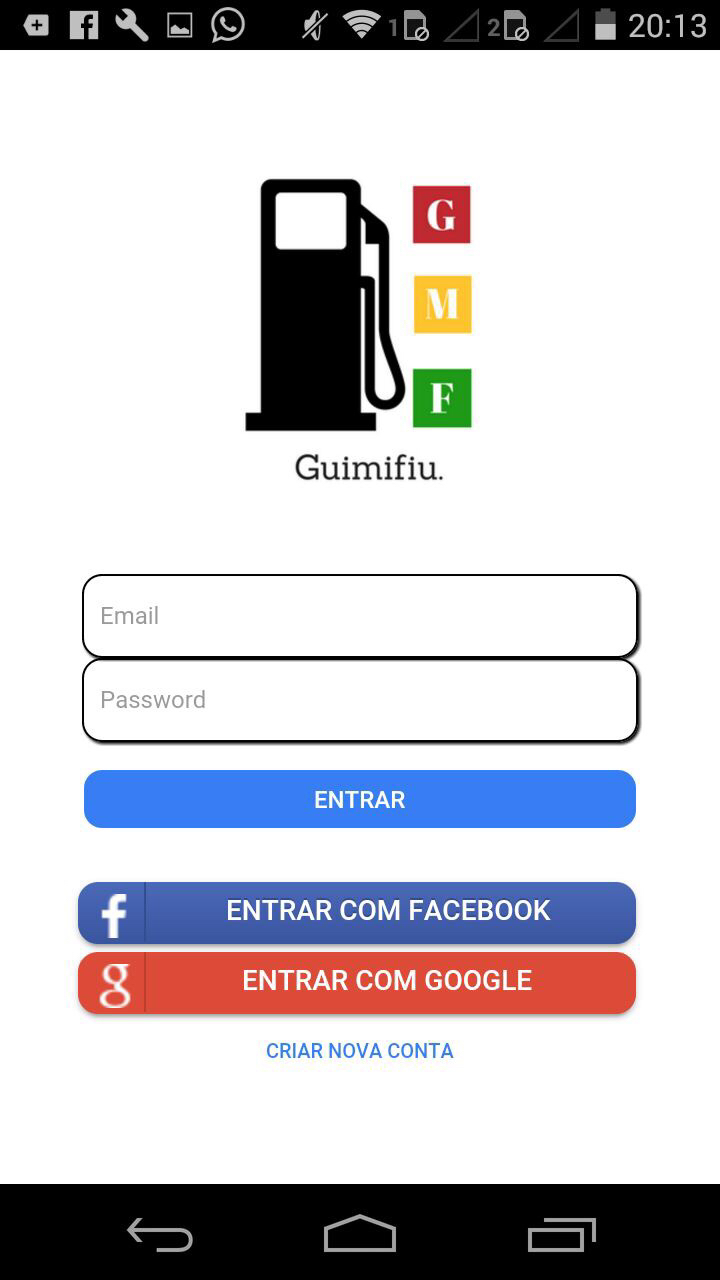
\includegraphics[scale=0.5]{figuras/app_1.jpg}
    \caption[Tela de login]{Tela de login. Fonte: autores}
    \label{img:tela_de_login}
\end{figure}

\begin{figure}[H]
    \centering
    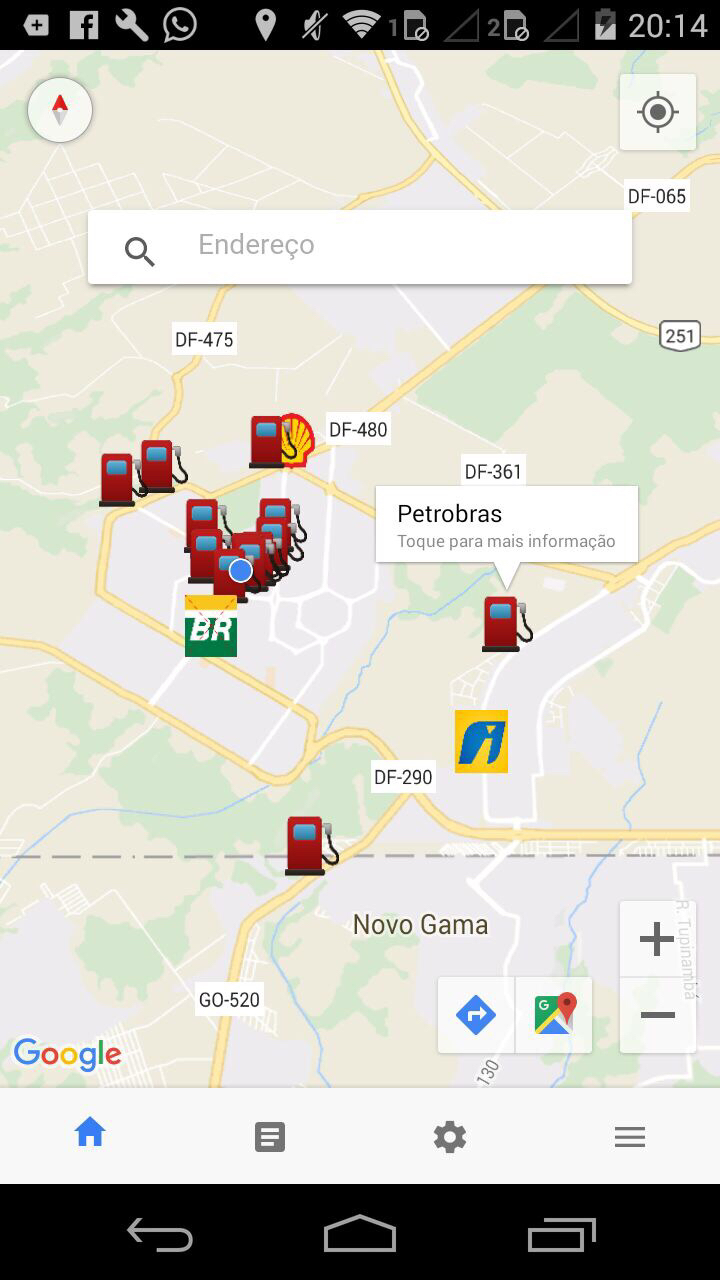
\includegraphics[scale=0.5]{figuras/app_2.jpg}
    \caption[Postos de gasolina próximos]{Postos de gasolina próximos. Fonte: autores}
    \label{img:postos_de_gasolina_próximos}
\end{figure}

\begin{figure}[H]
    \centering
    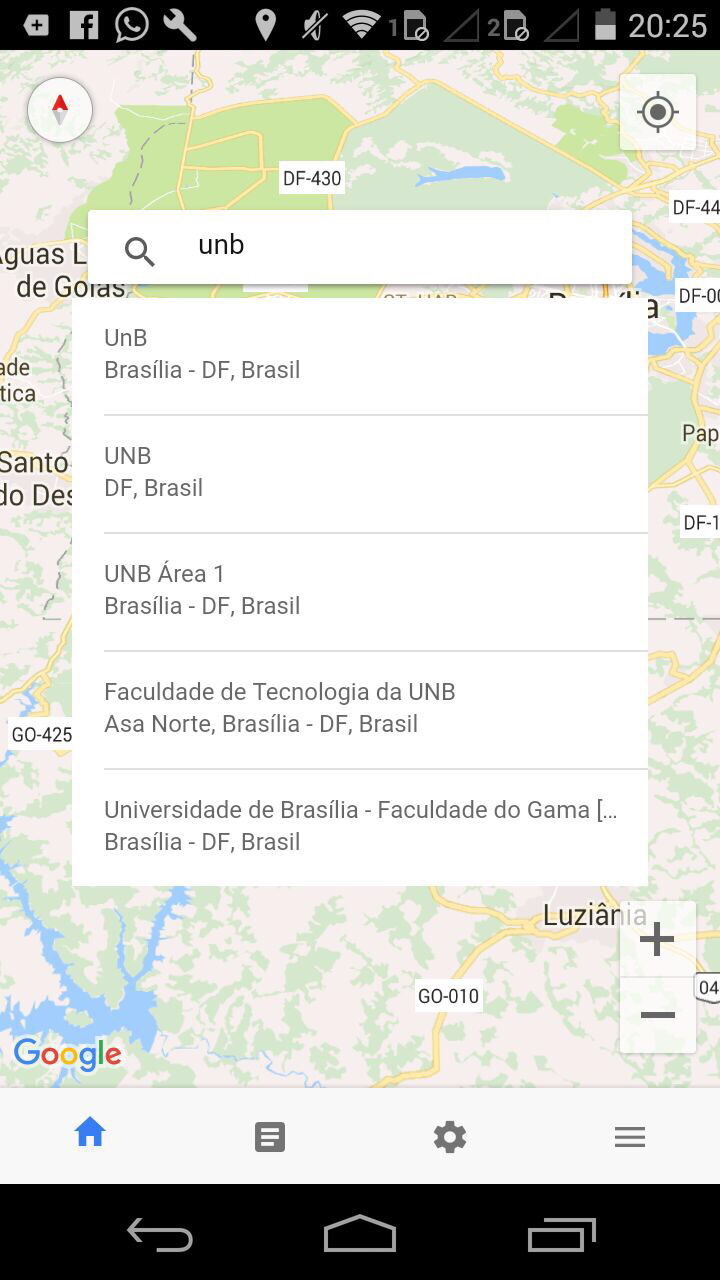
\includegraphics[scale=0.5]{figuras/app_3.jpg}
    \caption[Buscando localizações]{Buscando localizações. Fonte: autores}
    \label{img:buscando_localizacoes}
\end{figure}

\begin{figure}[H]
    \centering
    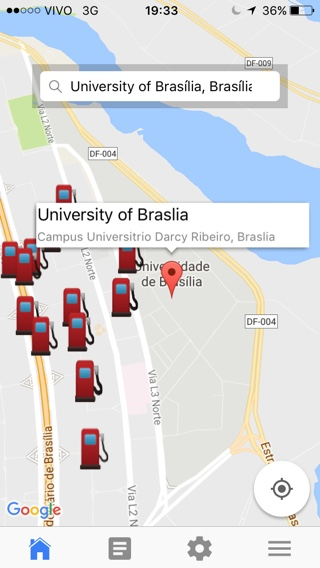
\includegraphics[scale=0.5]{figuras/app_4.jpg}
    \caption[Localização encontrada]{Localização encontrada. Fonte: autores}
    \label{img:localizacao_encontrada}
\end{figure}

\begin{figure}[H]
    \centering
    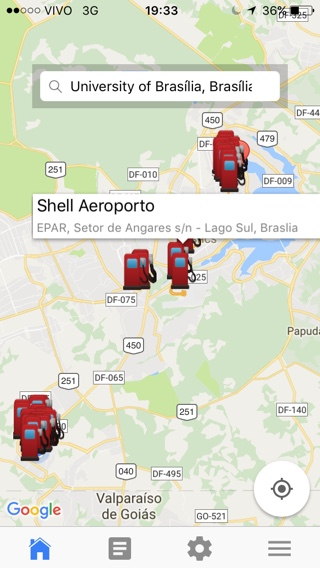
\includegraphics[scale=0.5]{figuras/app_5.jpg}
    \caption[Postos de gasolina próximos em uma rota]{Postos de gasolina próximos em uma rota. Fonte: autores}
    \label{img:postos_de_gasolina_proximos_em_uma_rota}
\end{figure}

\chapter{Coleta de Métricas}
\label{chap:metricas}

A figura \ref{img:rubocop} mostra o resultado da análise feita pelo rubocop. O arquivo de configuração utilizado para a análise pode ser encontrado \href{https://github.com/Guimifiu/guimifiu-backend/blob/master/.rubocop_config.yml}{aqui}.

\begin{figure}[H]
    \centering
    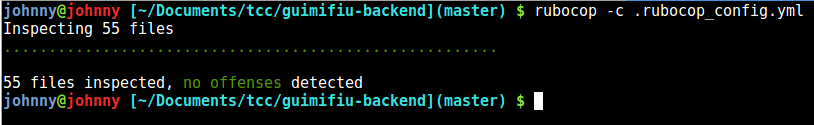
\includegraphics[scale=0.5]{figuras/rubocop.png}
    \caption[Relatório de análise estática do Rubocop]{Relatório de análise estática do Rubocop. Fonte: autores}
    \label{img:rubocop}
\end{figure}

A figura \ref{img:codeclimate} mostra o resultado das análises realizado pelo \href{https://codeclimate.com/github/Guimifiu/guimifiu-backend/}{CodeClimate}. 

\begin{figure}[H]
    \centering
    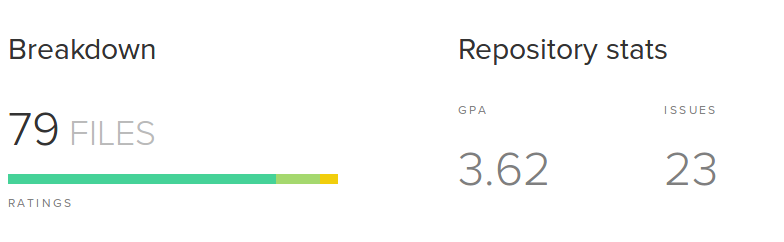
\includegraphics[scale=0.5]{figuras/codeclimate.png}
    \caption[Relatório de análise estática do CodeClimate]{Relatório de análise estática do CodeClimate. Fonte: autores}
    \label{img:codeclimate}
\end{figure}

Seis das sete \textit{issues} encontradas foram por motivo do CodeClimate utilizar um parser com uma versão menor do que a versão do Ruby utilizada pela equipe, enquanto a última foi uma duplicação de código que será tratada durante a segunda parte do trabalho.

\end{anexosenv}
